\chapter{Link-Cut Trees}

In this chapter, we will learn about a dynamic data structure that allows us to speed-up Dinic's algorithm even more: \emph{Link-Cut Trees}.

\section{Overview}

\paragraph{Model.} We consider a directed graph $G=(V,E)$ that is undergoing \emph{updates} in the form of edge insertions and/or deletions. We number the graph in its different \emph{versions} $G^0, G^1, G^2, \dots$ such that $G^0$ is the initial input graph, and $G^i$ is the initial graph after the first $i$ updates were applied. Such a graph is called a \emph{dynamic} graph.

In this lecture, we restrict ourselves to \emph{dynamic rooted forests} that is we assume that every $G^i$ forms a directed forest where in each forest a single root vertex is reached by every other vertex in the tree. For simplicity, we assume that $G^0 = (V, \emptyset)$ is an empty graph.

\begin{figure}[!ht]
    \centering
    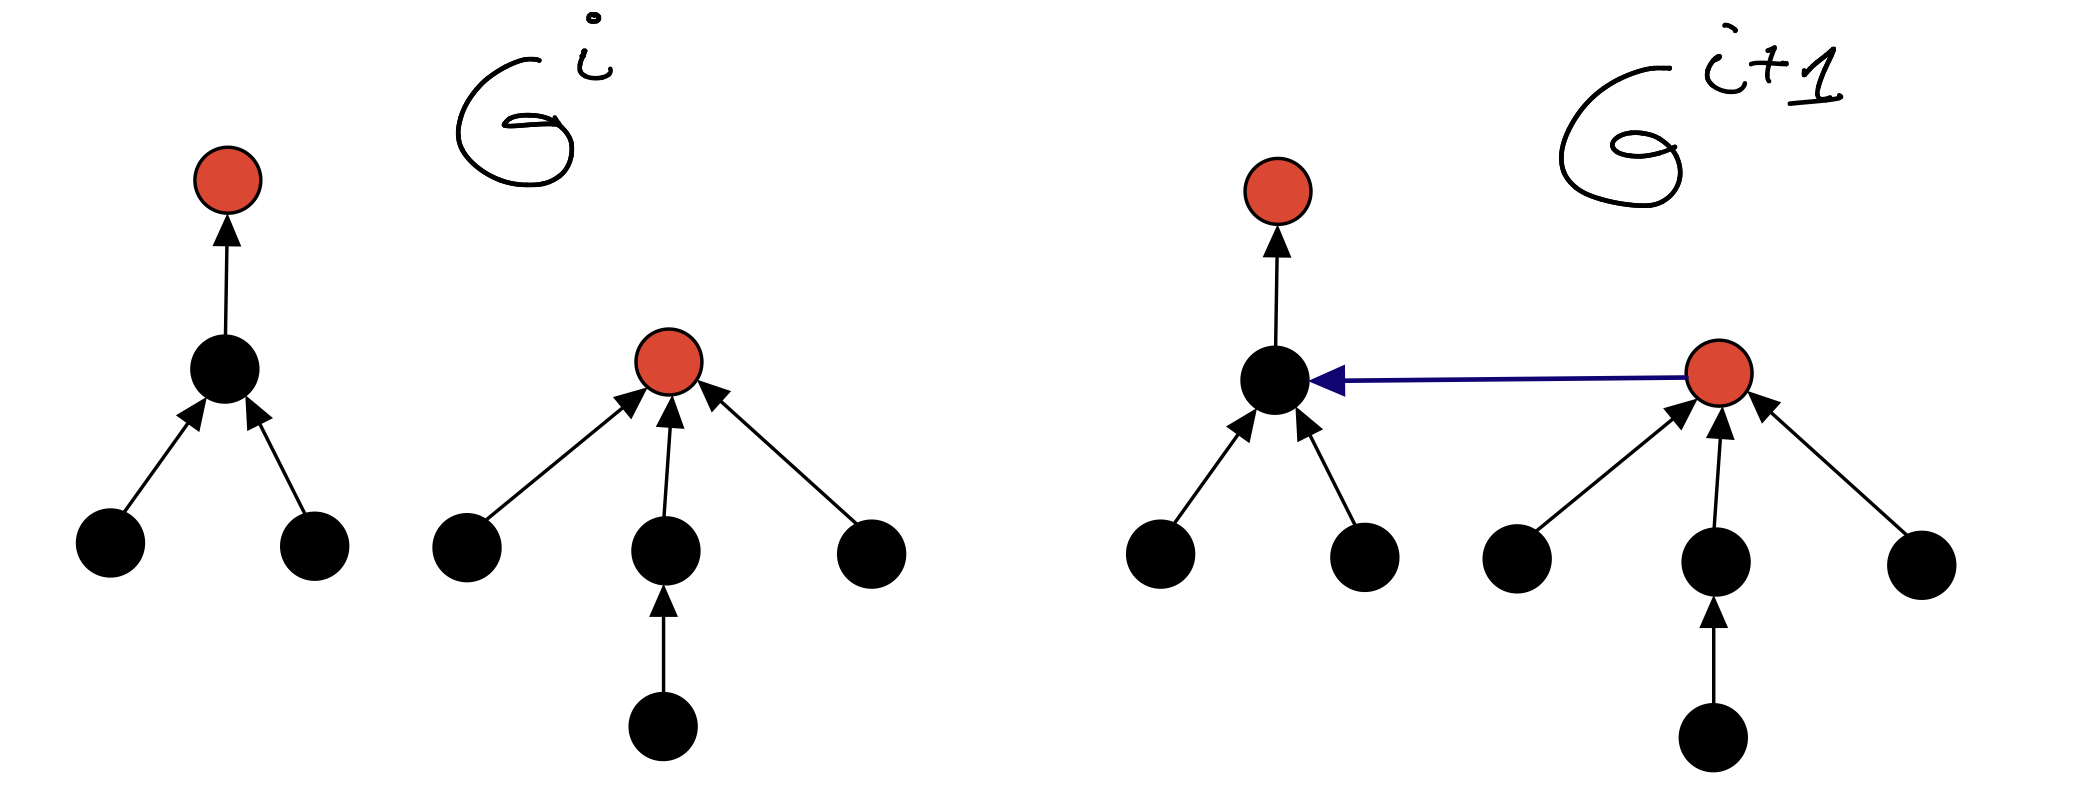
\includegraphics[scale=0.2]{./fig/InsertionDynamicTree_lectureDynamicTree.jpeg}
    \caption{The $i^{th}$ version of $G$ is a rooted forest. Here, red vertices are roots and there are two trees. The $(i+1)^{th}$ version of $G$ differs from $G^i$ by a single edge that was inserted (the blue edge). Note that edge insertions are only valid if the tail of the edge is a root.}
    \label{fig:my_label}
\end{figure}

\paragraph{The Interface.} Let us now describe the interface of our data structure that we call a link-cut tree. We want to support the following operations:
\begin{itemize}
    \item $\textsc{Initialize}(G)$: Creates the data structure initially and returns a pointer to it. Each vertex is initialized to have an associated cost $cost(v)$ equal to $0$.
    \item $\textsc{FindRoot}(v)$: Returns the root of vertex $v$. 
    \item $\textsc{AddCost}(v, \Delta)$: Add $\Delta$ to the cost of every vertex on the path from $v$ to the root vertex $\textsc{FindRoot}(v)$.
    \item $\textsc{FindMin}(v)$: Returns tuple $(w, cost(w))$ where $w$ is the (first) vertex on the path from $v$ to $\textsc{FindRoot}(v)$ of lowest cost. 
    \item $\textsc{Link}(u,v)$: Links two trees that contain $u$ and $v$ into a single tree by inserting the edge $(u,v)$. This assumes that $u, v$ are initially in different trees and $u$ was a root vertex.
    \item $\textsc{Cut}(u,v)$: Cuts the edge $(u,v)$ from the graph which causes the subtree rooted at $u$ to become a tree and $u$ to become a root vertex. Assumes $(u,v)$ is in the current graph.
\end{itemize}

\paragraph{Main Result.} The following theorem is the main result of today's lecture.

\begin{theorem}\label{thm:mainTheoremLinkCutTree}
We can implement a link-cut tree such that any sequence of $m$ operations takes total expected time $O(m \log^2 n + |V|)$.
\end{theorem}

\section{A Data Structure for Path Graphs}

Before we prove \Cref{thm:mainTheoremLinkCutTree} in its full generality, let us reason about implementing a link-cut tree data structure in a weaker setting: we assume that every version $G^i$ of $G$ is just a collection of rooted vertex-disjoint paths.

\paragraph{Representing Paths via Balanced Binary Search Trees.} It turns out that paths can be represented rather straight-forwardly via Balanced Binary Search Trees. For the sake of concreteness, we here use \emph{treaps} to represent paths\footnote{If you have not seen treaps before, don't worry, they are simple enough to understand them from our application here. }. 

Let us now describe how to represent a path $P$ in $G$. First, we pick for each vertex $v$, a random natural number $ranNum(v)$ uniformly at random from a large universe, say $[1, n^{100})$. We assume henceforth that $ranNum(v) \neq ranNum(w)$ for all $v,w\in V$.

Then, for each path $P$ in $G$, we store the vertices in $P$ in a binary tree $\mathcal{P}$ and enforce the invariants:
\begin{itemize}
    \item \textbf{Heap-Order}: for each vertex $v \in P$, its parent $w = parent_{\mathcal{P}}(v)$ in $\mathcal{P}$ is either $NULL$ (if $v$ is the root) or has $ranNum(v) > ranNum(w)$.
    \item \textbf{Search-Property}: for all $v$, $left_{\mathcal{P}}(v)$ precedes $v$ on $P$ and $right_{\mathcal{P}}(v)$ appears later on $P$ than $v$. See the picture below for an illustration.
\end{itemize}

\begin{figure}[!ht]
    \centering
    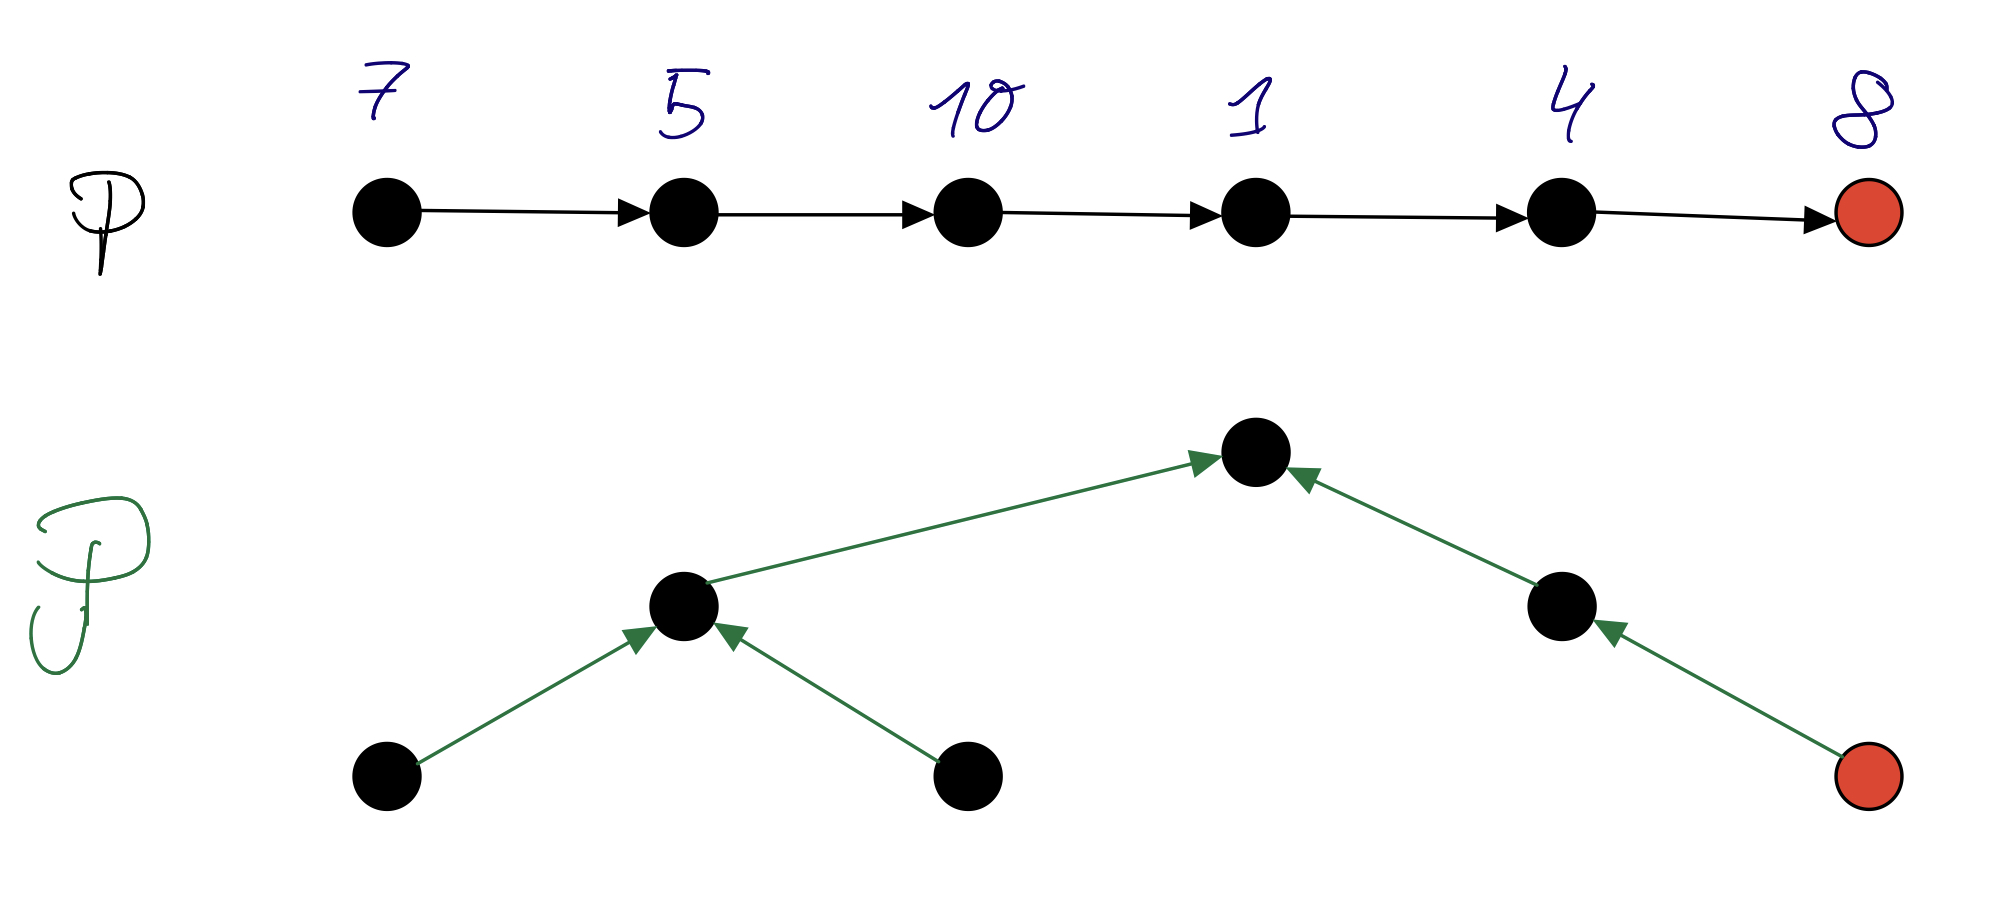
\includegraphics[scale=0.2]{./fig/PathRepTreap_lectureDynamicTree.jpeg}
    \caption{In the upper half of the picture, the original path $P$ in $G$ is shown, along with the random numbers $ranNum(v)$ for each $v$. The lower half depicts the resulting treap with vertices on the same vertical line as before.}
    \label{fig:my_label}
\end{figure}

\paragraph{Depth of Vertex in a Treap.} Let us next analyze the expected depth of a vertex $v$ in a treap $\mathcal{P}$ representing a path $P$. Let $P = \langle x_1, x_2, \dots, x_k = v, \dots, x_{|P|}\rangle$, i.e. $v$ is the $k^{th}$ vertex on the path $P$. Observe that a vertex $x_i$ with $i < k$ is an ancestor of $v$ in $\mathcal{P}$ if and only if no vertex $\{x_{i+1}, x_{i+2}, \dots, x_k\}$ has received a smaller random number than $ranNum(x_i)$. Since we sample $ranNum(w)$ uniformly at random for each $w$, we have that $\mathbb{P}[x_i \text{ ancestor of } v] = \frac{1}{k-i+1}$. The case where $i > k$ is analogous and has $\mathbb{P}[x_i \text{ ancestor of } v] = \frac{1}{i-k+1}$. Letting $X_i$ be the indicator variable for the event that $x_i$ is an ancestor of $v$, it is straight-forward to calculate the expected depth of $v$ in $\mathcal{P}$:
\[
    \mathbb{E}[depth(v)] = \sum_{i \neq k} \mathbb{E}[X_i] =  \sum_{i = 1}^{k-1}\frac{1}{k-i+1} + \sum_{i = k+1}^{|P|} \frac{1}{i-k+1} = H_k + H_{|P|-k+1} - 2 = O(\log |P|)
\]
It is straight-forward to see that the operation $\textsc{FindRoot}(v)$ can thus be implemented to run in expected $O(\log n)$ time by just iteratively following the parent pointers starting in $v$.

\paragraph{Implementing $\textsc{FindRoot}(v)$.} From any vertex $v$, we can simply follow the parent pointers in $\mathcal{P}$ until we are at the root of $\mathcal{P}$. Then, we find the right-most child of $\mathcal{P}$ by following the $left_{\mathcal{P}}$ pointers. Finally, we return the left-most child which is the root.

\paragraph{Implementing $\textsc{AddCost}(v, \Delta)$ and $\textsc{FindMin}(v)$.} The key trick to do the operations above efficiently is to store the change to subtrees instead of updating $cost(v)$ for each affected vertex. 

To this end, we store two fields $\Delta cost(v)$ and $\Delta min(v)$ for every vertex $v$. We let $cost(v)$ be the cost of each vertex, and $mincost(v)$ denote the minimum cost of any descendant of $v$ in $\mathcal{P}$. Then, we maintain for each $v$
\[
    \Delta cost(v) = cost(v) - mincost(v)
\]
\[
    \Delta min(v) = \begin{cases}
    mincost(v) & parent_{\mathcal{P}}(v) = NULL, \\
    mincost(v) - mincost(parent_{\mathcal{P}}(v)) & otherwise\end{cases}
\]
It is not hard to see that with these definitions, we obtain $mincost(v) = \sum_{w \in \mathcal{P}[v]} \Delta min(v)$ where $\mathcal{P}[v]$ is the $v$-to-root path in $\mathcal{P}$. We can then recover $cost(v) = mincost(v) + \Delta cost(v)$. 

To enforce this invariant, when $\textsc{AddCost}(v, \Delta)$ is invoked, we can simply manipulate the fields of vertices that are adjacent to the $v$-to-root path in $\mathcal{P}$ (This depends on whether the path takes a right or left turn). This can be done in expected $O(\log n)$ time.

To implement the operation $\textsc{FindMin}(v)$ efficiently, we can use binary search to visit a child $w$ (the left one if both are eligible) where $mincost(v) = mincost(w)$. It is not hard to see that each $mincost(w)$ can be found in $O(1)$ given the $mincost$ of its parent. Thus, one can implement $\textsc{FindMin}(v)$ again in $O(\log n)$ expected time.

\paragraph{Implementing $\textsc{Link}(u,v)$ and $\textsc{Cut}(u,v)$.} We start by showing how to implement $\textsc{Cut}(u,v)$. Therefore, we assume that we have a dummy node $d_0$ with $ranNum(d_0) = 0$ in the vertex set. The trick is to first treat the operation as splitting the edge $(u,v)$ into $(u,d_0)$ and $(d_0,v)$ by inserting the vertex $d_0$ in between $u$ and $v$ in the tree $\mathcal{P}$ as a leaf (this is always possible). Then, we can do standard binary tree rotations to re-establish the heap-order invariant (here we have to also carefully recompute the new fields we introduce but this can again be done in $O(1)$ time per rotation). It is not hard to see that after $O(\log n)$ tree rotations in expectation, the heap-order is re-established and $d_0$ is at new root of $\mathcal{P}$. It remains to remove $d_0$ and make $left_{\mathcal{P}}(d_0)$ and $right_{\mathcal{P}}(d_0)$ tree roots.

\begin{figure}[!ht]
    \centering
    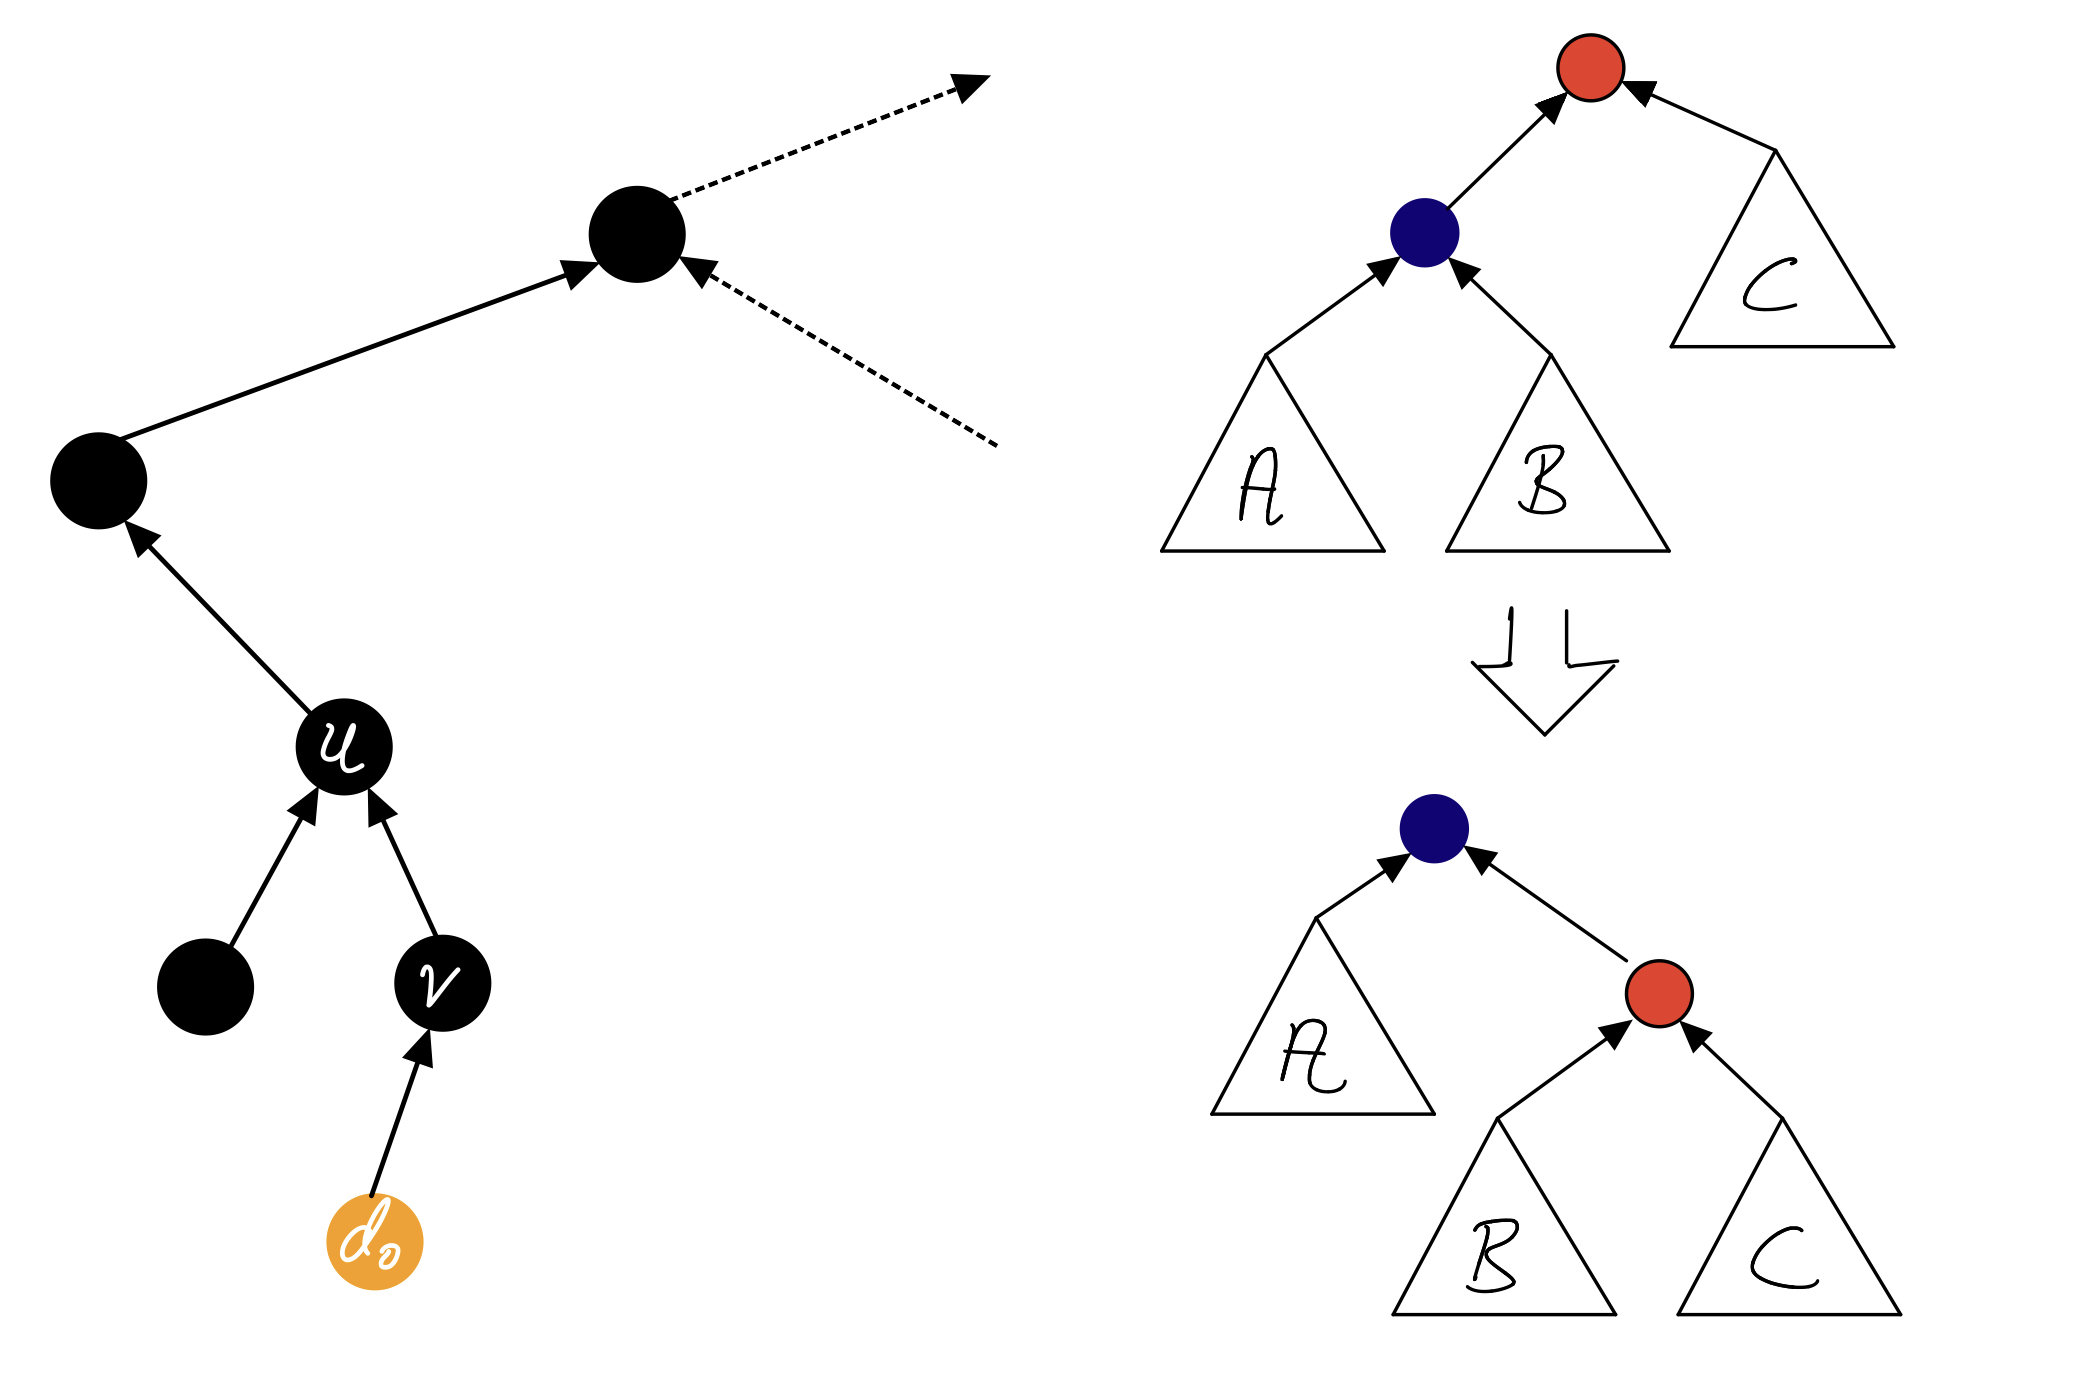
\includegraphics[scale=0.2]{./fig/PathCutOperation_lectureDynamicTree.jpeg}
    \caption{For $\textsc{Cut}(u,v)$, we insert a vertex $d_0$ as a leaf of either $u$ or $v$ to formally split $(u,v)$ into $(u,d_0)$ and $(d_0,v)$ (this is shown on the left). While this preserves that Search-Property, it will violate the Heap-Order. Thus, we need to use tree rotations (shown on the left) to push $d_0$ to the top of the tree $\mathcal{P}$ (the arrow between the tree rotations should point in both ways).}
\end{figure}

Implementing $\textsc{Link}(u,v)$ can be done by reversing this process, i.e. inserting a vertex $d_{\infty}$ with $ranNum(d_{\infty}) = n^{100}$ where we let $left_{\mathcal{P}}(d_{\infty})$ point to the root of the tree representing the path $u$ is currently contained in,  and  $right_{\mathcal{P}}(d_{\infty}) $ to the root of the tree over the path that $v$ is contained in (and adapt the parent pointers). Using rotations to enforce Heap-Order, we have $d_{\infty}$ as a leaf and can just remove it from the tree (which can be seen as un-splitting two edges into $(u,v)$).  Note that here,  we also have to carefully enforce the Search Property ourselves to ensure that $d_{\infty}$ is always in between $u$ and $v$ on the path.

\paragraph{Notes.} The operations $\textsc{Link}/ \textsc{Cut}$ can be implemented for almost all Balanced Binary Search Trees (especially the ones you have seen in your first courses on data structures). Thus, it is not hard to get a $O(\log n)$ worst-case time bound for all operations discussed above.

\section{Implementing Trees via Paths}

We now use the result from last section as a black box to obtain \Cref{thm:mainTheoremLinkCutTree}.

\paragraph{Path Decomposition.} For each rooted tree $T$, the idea is to decompose $T$ into paths. In particular, we decompose each $T$ into a collection of vertex-disjoint paths $P_1, P_2, \dots, P_k$ such that each internal vertex $v$ in $T$ has exactly one incoming edge in some $P_i$. We call the edges on some $P_i$  \emph{solid} edges and say that the other edges are \emph{dashed}. 

We maintain the paths $P_1, P_2, \dots, P_k$ using the data structure described in the last section. To avoid confusion, we use the prefix $P$ when we invoke operations of the path data structure, for example $\textsc{PFindRoot}(v)$ finds the root of $v$ in the path graph consisting of all the $P_i$'s.

\begin{figure}[!ht]
    \centering
    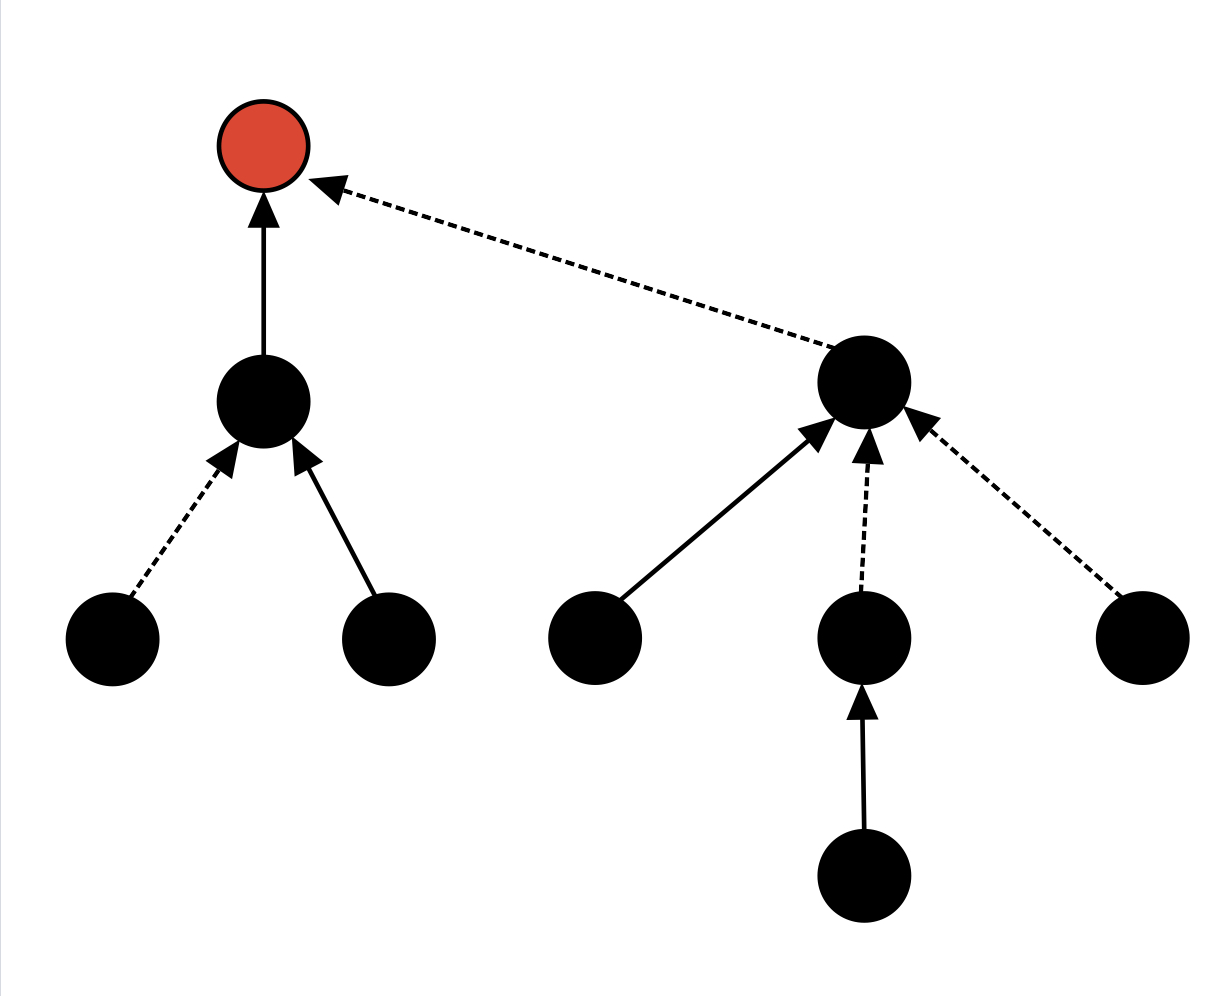
\includegraphics[scale=0.20]{./fig/HeavyLightDecomposition_lectureDynamicTree.jpeg}
    \caption{The dashed edges are the edges not on any path $P_i$. The collection of (non-empty) paths $P_1, P_2, \dots, P_k$ can be seen to be the maximal path segments of solid edges.}
\end{figure}

\paragraph{The $\textsc{Expose}(v)$ Operation.} We now discuss the most important operation of the data structure that will be used by all other operations internally: the operation $\textsc{Expose}(v)$. This operation flips solid/dashed edges such that after the procedure the path from $v$ to its tree root in $G$ is solid (possibly as a subpath in the path collection). Below you can find an implementation of the procedure $\textsc{Expose}(v)$. 

\begin{algorithm}
  \SetAlgoLined
  $w \gets v$.\\
  \While{$(w' = parent_G(\textsc{PFindRoot}(w))) \neq NULL$}{
    Invoke $\textsc{PCut}(z,w')$ for the solid edge $(z,w')$ incoming to $w'$.\\
    $\textsc{PLink}(w,w')$.\\
    $w \gets w'$.\\
  }
  \caption{\textsc{Expose}(v)}
\end{algorithm}

\paragraph{Implementing Operations via $\textsc{Expose}(v)$.} We can now implement link-cut tree operations by invoking $\textsc{Expose}(v)$ and then forwarding the operation to the path data structure. 
\begin{algorithm}[H]
  \SetAlgoLined
  $\textsc{Expose}(v)$; $\textsc{PAddCost}(v, \Delta)$
  \caption{$\textsc{AddCost}(v, \Delta)$}
\end{algorithm}
\begin{algorithm}[H]
  \SetAlgoLined
  $\textsc{Expose}(v)$; \Return $\textsc{PFindMin}(v)$
  \caption{\textsc{FindMin}(v)}
\end{algorithm}
\begin{algorithm}[H]
  \SetAlgoLined
  $parent_G(u) \gets v$\;
  \lIf{$v$ has an incoming solid edge $(z,v)$}{
    $\textsc{PCut}(z,v)$
  }
  $\textsc{PLink}(u,v)$
  \caption{\textsc{Link}(u,v)}
\end{algorithm}
\begin{algorithm}[H]
  \SetAlgoLined
  $\textsc{Expose}(u)$; $parent_G(u) \gets NULL$; $\textsc{PCut}(u,v)$\;
   \lIf{$v$ has other incoming edge $(z,v)$}{$\textsc{PLink}(z,v)$}
  \caption{\textsc{Cut}(u,v)}
\end{algorithm}

\paragraph{Analysis.} All of the operations above can be implemented using a single $\textsc{Expose}(\cdot)$ operation plus $O(1)$ operations on paths. Since path operations can be executed efficiently, our main task is to bound the run-time of $\textsc{Expose}(\cdot)$. More precisely, since each iteration of $\textsc{Expose}(\cdot)$ also runs in time $O(\log n)$, the total number of while-loop iterations in $\textsc{Expose}(\cdot)$.

To this end, we introduce a dichotomy over the vertices in $G$. We let $parent_G(v)$ denote the unique parent of $v$ in $G$ and let $size_G(v)$ denote the number of vertices in the subtree rooted at $v$ (including $v$). 

\begin{definition}
Then, we say that an edge $(u,v)$ is \emph{heavy} if $size_G(u) > size_G(v)/2$. Otherwise, we say $(u,v)$ is \emph{light}. 
\end{definition}

It can now be seen that the number of \emph{light} edges on the $v$-to-root path for any $v$ is at most $\lg n$: every time we follow a light edge $(w,w')$, i.e. when $size_G(w') > 2 size_G(w)$, we double the size of the subtree so after taking more than $\lg n$ such edges, we have $> 2^{\lg n} = n$ vertices in the graph (which is a contradiction).

Thus, when $\textsc{Expose}(\cdot)$ runs for many iterations, it must turn many \emph{heavy} edges \emph{solid} (this is also since each vertex has at most one incoming heavy edge, so when we make a heavy edge solid, we also don't make any other heavy edge solid). 

\begin{claim}
Each update can only increase the number of dashed, heavy edges by $O(\log n)$. 
\end{claim}
\begin{proof}
First observe that every time $\textsc{Expose}(\cdot)$ is invoked, it turns at most $\lg n$ heavy edges from solid to dashed (since it has to visit a light edge to do so).

The only two operations that can cause additional dashed, heavy edges are $\textsc{Link}(u,v)$ and $\textsc{Cut}(u,v)$ by toggling heavy/light. For $\textsc{Link}(u,v)$, we observe that only the vertices on the $v$-to-root path increase their sizes. Since there are at most $\lg n$ light edges on this path that can turn heavy, this increases the number of dashed, heavy edges by at most $\lg n$. 

The case for $\textsc{Cut}(u,v)$ is almost analogous: only vertices on the $v$-to-root path decrease their sizes which can cause any heavy edge on such a path to become light, and instead for a sibling of such a vertex might becomes heavy. But there can be at most $\lg n$ such new heavy edges, otherwise the total size of the tree must exceed again $n$ which leads to a contradiction.
\end{proof}

We conclude that the while-loop in $\textsc{Expose}(\cdot)$ runs for at most $O(m \log n)$ iterations after $m$ updates. Each iteration can be implemented in $O(\log n)$ expected time. This dominates the total running time and proves \Cref{thm:mainTheoremLinkCutTree}.

\section{Fast Blocking Flow via Dynamic Trees}

Recall from \Cref{sec:findBlockingFlows} that computing blocking flows in a level graph $L$ from a vertex $s$ to $t$ can be done by successively running $\textsc{DFS}(s)$ and routing flow along the $s$-$t$ path found if one such path exists and otherwise we know that we have found a blocking flow. 

We can now speed-up this procedure by storing the DFS-tree explicitly as a dynamic tree. To simplify exposition, we transform $L$ to obtain a graph $\textsc{Transform}(L)$ that has capacities on vertices instead of edges. To obtain $\textsc{Transform}(L)$, we simply split each edge in $L$ and assign the edge capacity to the mid-point vertex while assigning capacity $\infty$ to all vertices that were already in $L$. This creates an identical flow problem with at most $O(m)$ vertices and edges.

\begin{figure}[!ht]
    \centering
    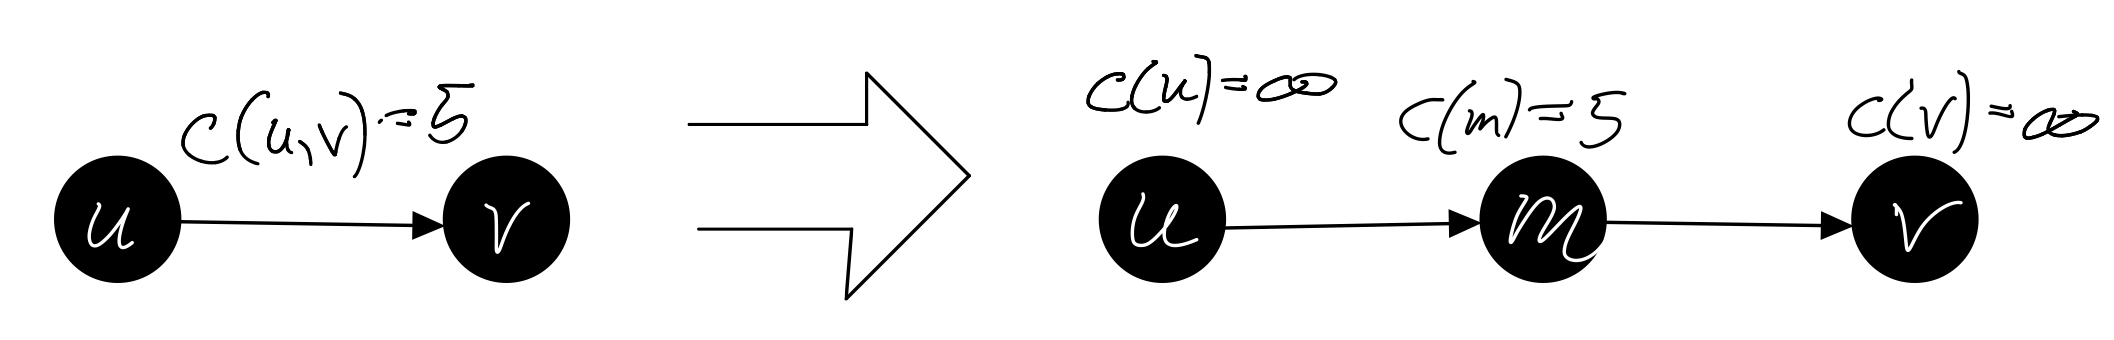
\includegraphics[scale=0.2]{./fig/TransformToVertCaps_lectureDynamicTree.jpeg}
    \caption{Each edge $(u,v)$ with capacity $c(u,v)$ is split into two edges $(u,m)$ and $(m,v)$. The capacity is then on the vertex $m$.}
    \label{fig:my_label}
\end{figure}

Finally, we give the new pseudo-code for the blocking flow procedure below.

\begin{algorithm}[H]
  \SetAlgoLined
  $H \leftarrow \textsc{Transform}(L)$\;
  $\textsc{LC-Tree} \gets \textsc{Initialize}(H)$\;
  
  \While{$s \in H$}{
    $u \gets \textsc{LC-Tree}.\textsc{FindRoot}(s)$\;
    \eIf{there is an edge $(u,v) \in H$}{
        $\textsc{LC-Tree}.\textsc{Link}(u,v)$\;
        \If{$v = t$}{
            $(w, c) \gets \textsc{LC-Tree}.\textsc{FindMin}(s)$\;
            $\textsc{LC-Tree}.\textsc{AddCost}(s, - c)$\;
            Remove $w$ and all its incident edges from $H$ and $\textsc{LC-Tree}$ (via $\textsc{Cut}(\cdot)$).
        }
    }{
        Remove $u$ and all its incident edges from $H$ and $\textsc{LC-Tree}$ (via $\textsc{Cut}(\cdot)$).
    }
  }
  Construct $\ff$ by setting for each edge $(u,v)$ of $L$, with mid-point $m$ in $\textsc{Transform}(L)$, the flow equal to $c(m)$ minus the cost on $m$ just before it was removed from $H$.
  \caption{\textsc{FindBlockingFlow}(s, t, L)}
\end{algorithm}

\begin{claim}
The running time of $\textsc{FindBlockingFlow}(s, t, L)$ is $O(m \log^2 n + |V|)$.
\end{claim}
\begin{proof}
Each edge $(u,v)$ in the graph $\textsc{Transform}(L)$ enters the link-cut tree at most once (we only invoke $\textsc{Cut}(u,v)$ when we delete $(u,v)$ from $H$). 

Next, observe that the first $if$-case requires $O(1 + \#edgesDeletedFromH)$ many tree operations. The $else$-case requires $O(\#edgesDeletedFromH)$ many tree operations. 

But each edge is only deleted once from $H$, thus we have a total of $O(m)$ tree operations over all iterations. Since each link-cut tree operation takes amortized expected time $O(\log^2 n)$, we obtain the bound on the total running time. 
\end{proof}

The correctness of this algorithm follows almost immediately using that the level graph $L$ (and therefore $\textsc{Transform}(L)$) is an ayclic graph.

%%% Local Variables:
%%% mode: latex
%%% TeX-master: "agao21_script"
%%% End: